\documentclass[3p,times,procedia]{elsarticle}


\flushbottom

%% The `ecrc' package must be called to make the CRC functionality available
\usepackage{ecrc}
%\usepackage{amsmath}


%% The ecrc package defines commands needed for running heads and logos.
%% For running heads, you can set the journal name, the volume, the starting page and the authors

%% set the volume if you know. Otherwise `00'
\volume{00}

%% set the starting page if not 1
\firstpage{1}

%% Give the name of the journal
\journalname{24th EURO Working Group on Transportation Meeting, EWGT 2021, 8-10 September 2021, Aveiro, Portugal}

%% Give the author list to appear in the running head
%% Example \runauth{C.V. Radhakrishnan et al.}
\runauth{A. Nacer-Weill, C. Yang, T. Barbet and J Raimbault}

%% The choice of journal logo is determined by the \jid and \jnltitlelogo commands.
%% A user-supplied logo with the name <\jid>logo.pdf will be inserted if present.
%% e.g. if \jid{yspmi} the system will look for a file yspmilogo.pdf
%% Otherwise the content of \jnltitlelogo will be set between horizontal lines as a default logo

%% Give the abbreviation of the Journal.
\jid{trpro}

%% Give a short journal name for the dummy logo (if needed)
%\jnltitlelogo{Transportation Research}

%% Hereafter the template follows `elsarticle'.
%% For more details see the existing template files elsarticle-template-harv.tex and elsarticle-template-num.tex.

%% Elsevier CRC generally uses a numbered reference style
%% For this, the conventions of elsarticle-template-num.tex should be followed (included below)
%% If using BibTeX, use the style file elsarticle-num.bst

%% End of ecrc-specific commands
%%%%%%%%%%%%%%%%%%%%%%%%%%%%%%%%%%%%%%%%%%%%%%%%%%%%%%%%%%%%%%%%%%%%%%%%%%

%% The amssymb package provides various useful mathematical symbols

\usepackage{amssymb}
%% The amsthm package provides extended theorem environments
%% \usepackage{amsthm}

%% The lineno packages adds line numbers. Start line numbering with
%% \begin{linenumbers}, end it with \end{linenumbers}. Or switch it on
%% for the whole article with \linenumbers after \end{frontmatter}.
%% \usepackage{lineno}

%% natbib.sty is loaded by default. However, natbib options can be
%% provided with \biboptions{...} command. Following options are
%% valid:

%%   round  -  round parentheses are used (default)
%%   square -  square brackets are used   [option]
%%   curly  -  curly braces are used      {option}
%%   angle  -  angle brackets are used    <option>
%%   semicolon  -  multiple citations separated by semi-colon
%%   colon  - same as semicolon, an earlier confusion
%%   comma  -  separated by comma
%%   numbers-  selects numerical citations
%%   super  -  numerical citations as superscripts
%%   sort   -  sorts multiple citations according to order in ref. list
%%   sort&compress   -  like sort, but also compresses numerical citations
%%   compress - compresses without sorting
%%
\biboptions{authoryear}

% \biboptions{}

% if you have landscape tables
\usepackage[figuresright]{rotating}
%\usepackage{harvard}
% put your own definitions here:x
%   \newcommand{\cZ}{\cal{Z}}
%   \newtheorem{def}{Definition}[section]
%   ...

% add words to TeX's hyphenation exception list
%\hyphenation{author another created financial paper re-commend-ed Post-Script}

% declarations for front matter

\usepackage[bookmarks=false]{hyperref}
    \hypersetup{colorlinks,
      linkcolor=blue,
      citecolor=blue,
      urlcolor=blue}

\usepackage{multicol}




\begin{document}
\begin{frontmatter}

%% Title, authors and addresses

\title{An agent-based model for modal shift in public transport}

\author[a]{Amine Nacer-Weill}
\author[a]{Changtao Yang}
\author[a]{Thibaut Barbet}
\author[b]{Juste Raimbault\corref{cor1}}

\address[a]{Ecole des Ponts ParisTech, Champs-sur-Marne, France}
\address[b]{CASA, University College London, London, United Kingdom}

\begin{abstract}
Modal shift in public transport as a consequence of a disruption on a line has in some cases unforeseen consequences such as an increase in congestion in the rest of the network. How information is provided to users and their behavior plays a central role in such configurations. We introduce here a simple and stylised agent-based model aimed at understanding the impact of behavioral parameters on modal shift. The model is applied on a case study based on a stated preference survey for a segment of Paris suburban train network. We systematically explore the parameter space and show non-trivial patterns of congestion for some values of discrete choice parameters linked to perceived wait time and congestion. Work in progress include the application of optimization algorithms to the model to search for optimal compromises between congestion in different modes.
\end{abstract}

\begin{keyword}
Modal shift \sep Public transport disruption \sep Agent-based modeling \sep Model exploration
\end{keyword}
\cortext[cor1]{Corresponding author.}
\end{frontmatter}

\email{j.raimbault@ucl.ac.uk}

%%
%% Start line numbering here if you want
%%
% \linenumbers

%% main text

%\enlargethispage{-7mm}
%\section{Introduction}


%Dans les transports en communs aussi les usagers doivent faire des choix en un temps limité et avec des informations limitées. Ils subissent régulièrement des perturbations. Il s’enclenche alors un processus de décision complexe qui va aboutir à des comportements complexes. Le travail de Xavier Brisbois1 notamment a contribué à montrer que l'analyse choix de report modal à long terme ne peut se dispenser d'une analyse des comportements, de la dimension cognitive du choix en complément de variables socio-économiques qui n’expliquentpas nécessairement les comportements.
%En s’inspirant des modèles d’information voyageur comme ceux de Leng et Corman2 qui explorent les effets de l’information voyageur sur les temps de trajet, nous nous posons la question de la complémentarité de ces modélisations multiagents avec des enquêtes de préférences déclarées. 

Disruptions in public transport networks are not rare events, often worsened by an increased complexity of these networks and their management \citep{dekker2018next}. Network resilience is then tightly linked to patterns of modal shift \cite{stamos2015impact}, and a better understanding of these is crucial both from a theoretical and operational viewpoint. In that context, users have to make decisions in a limited time and under partial information. The study of modal shift under disruption is therefore improved when taking into account users behavior and a detailed representation of users cognition \citep{brisbois2010processus}. More particularly, the role of information provided in real time can in some cases become crucial, as rerouting may in fact increase the congestion in other parts of the network and ultimately increase the average travel time \citep{chatterjee2002driver,chorus2006travel}.

To study mechanisms linking information given to users with modal shift, and more generally the evolution of multi-modal network flows under disruptions, agent-based modeling has been highlighted as a relevant approach \citep{leng2020role}. For example, \cite{leng2020issue} show that the issue time of information has a significant impact on the total congestion. Agent-based models are used in similar studies of modal share, such as by \cite{baindur2011agent} for freight. \cite{raney2003agent} describe an application of the Matsim model, which is a data-driven agent-based and activity-based transport model, to a large sample of Switzerland transport network. The Matsim model can be applied at large scales in a reproducible manner, such as in the case of Ile-de-France illustrated by \cite{horl2020reproducible}.

Large transport agent-based models such as Matsim however require an extensive parametrisation on real data, are difficult to systematically validate given their runtime and large parameter space, and despite their high modularity can be tuned only to some extent regarding a precise description of users behavior in public transport and their interactions with a network disruption. This paper therefore proposes to introduce a simple and stylised agent-based model to understand the role of information and user behavior in modal shift under disruptions in public transport. With a reduced computational complexity but also parameter space to explore, under limited requirements for data, such a model can be used to systematically explore if some qualitative stylised facts are robustly found under different scenario, and possibly extended into a decision-making tool. Our contribution is threefold: (i) we contextualize the construction of the model with a reduced stated preferences survey, applied on a case study in the Parisian public transport network on a specific segment often subject to disruption; (ii) we introduce the simple agent-based model as an open-source tool, which can be extended or modified to test concurrent hypotheses on user behavior; (iii) we proceed to a systematic exploration of the model parameter space, unveiling some non-linear patterns and a counter-productive reaction of users to the disruption in terms of congestion for some scenarios.


%\section{Stated preferences survey}

%Notre but est de déterminer si l’accès à l’information sur le temps d’attente lors d’une perturbation pour les usagers est utile ou non. Pour commencer nous établissons un périmètre d’étude. Dans notre cas nous nous intéressons au RER A, il nous faut cependant réduire notre périmètre pour nous concentrer sur une zone plus précise. Nous souhaitons vérifier l’impact sur le réseau, pour cela nous choisissons donc des stations qui soient suffisamment maillées entre elles pour pouvoir dessiner un “mini-réseau”. Le but est de construire notre étude pour un trajet s’effectuant d’un point A à un point B. De plus, afin de s’assurer que les usagers effectuent le trajet qui nous intéresse, et par simplification de notre “mini-réseau”, nous devons choisir deux stations proches l’une de l’autre. Nous étudierons donc ici le report modal (ou le reroutage) en cas de situation perturbée sur la ligne du RER.

We first proceeded to a small size stated preferences survey %\citep{kroes1988stated}
, in order to have a qualitative overview of processes needed in the model and to have a case study for model application. \cite{martin2016strategies} have indeed shown that there exists a high heterogeneity in user reaction to disruptions. We choose to study the line A of the \emph{RER} suburban train in Paris, which has the highest load in the region and has a non negligible frequency of disruption. We focus on a subpart of the network, in order to sample users which have a higher chance of realizing a given origin-destination pattern, and for which several modal alternatives exist. Therefore, the segment \emph{Etoile-La Defense} was chosen, as it features alternative trips with the \emph{Metro Line 1} and several bus lines.


%%%%%%%%%%%%
\begin{figure}[t]\vspace*{4pt}
\centerline{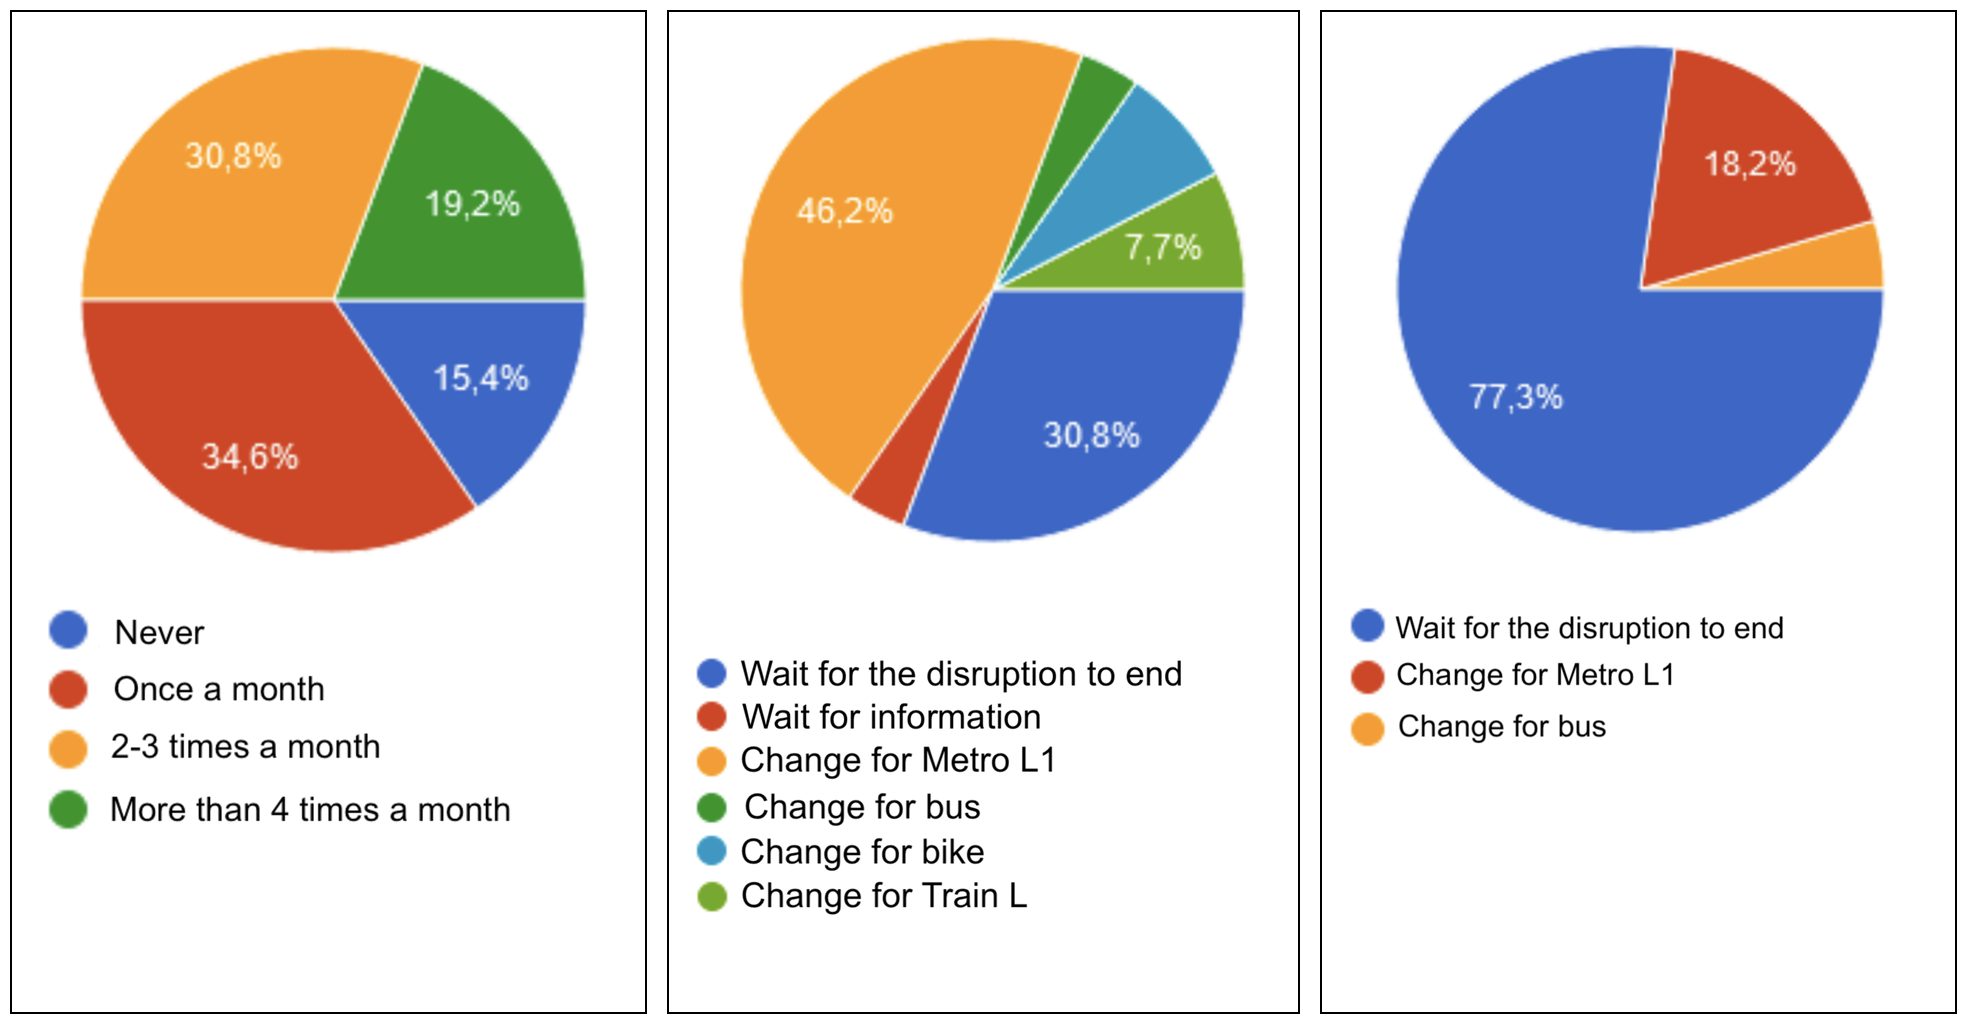
\includegraphics[width=0.45\linewidth]{figures/Fig1.png}}
\caption{Results of the declared preference survey. \textit{(Left)} Number of times a month users experience a disruption; \textit{(Middle)} Behavior of users when no information is given; \textit{(Right)} Behavior of users when a 10 minutes traffic stop is announced.\label{fig:fig1}}
\end{figure}
%%%%%%%%%%%%

We surveyed a total of $N=48$ users, among which a subsample of $N=27$ were regular users for which the full questionnaire was given. Main results which can inform our model context are shown in Fig.~\ref{fig:fig1}. We first confirm that disruptions are indeed frequent on the line, as around 50\% of users experience a disruption at least twice a month. We then find that under no information, user behavior is heterogeneous and a large part shifts to alternative itineraries. Finally, when users are informed of a 10 minutes disruption, on the contrary more than 75\% decide to wait on place. Therefore, the model must include various modal shifts, but also take into account how perceived wait time will influence user choice.



%\section{Model description and exploration}

The agent-based model is based on two types of agents: users and RER trains. The simulated segment of the network is included for the main mode (RER train) and alternative modes (metro, bus, taxi, bike, walking). Main mode is simulated in full granularity, i.e. including train boarding, train capacity and train alighting. Other modes are simulated as queues with a given capacity. One simulation covers peak hours (180 time steps) with stationary Poisson arrival of users for each mode. At each time step: (i) users waiting for a train evaluate a discrete choice utility difference (between waiting and shifting to an other mode) given by $U_i = \beta_c \cdot c + \beta_{\tau} \tau$ where $c$ is perceived congestion given by the current number of user waiting (normalized by platform capacity) and $\tau$ is perceived time proportional to user current travel time (time since departure) and current waiting time between trains, and switch mode accordingly with a probability of $p_i = 1 / (1 + \exp \Delta U_i)$ and with fixed probabilities across other modes; (ii) next train possibly enter station and users board at a given speed and given train capacity, while users alights at the end of the segment if a train is in station; (iii) train queue on the segment is simulated with proper speeds; (iv) other modes are simulated as queues with a given user capacity. Model results are assessed with indicators giving the average travel time and average congestion over the peak hour and all users.

%%%%%%%%%%%%%
%\begin{figure}[t]\vspace*{4pt}
%\centerline{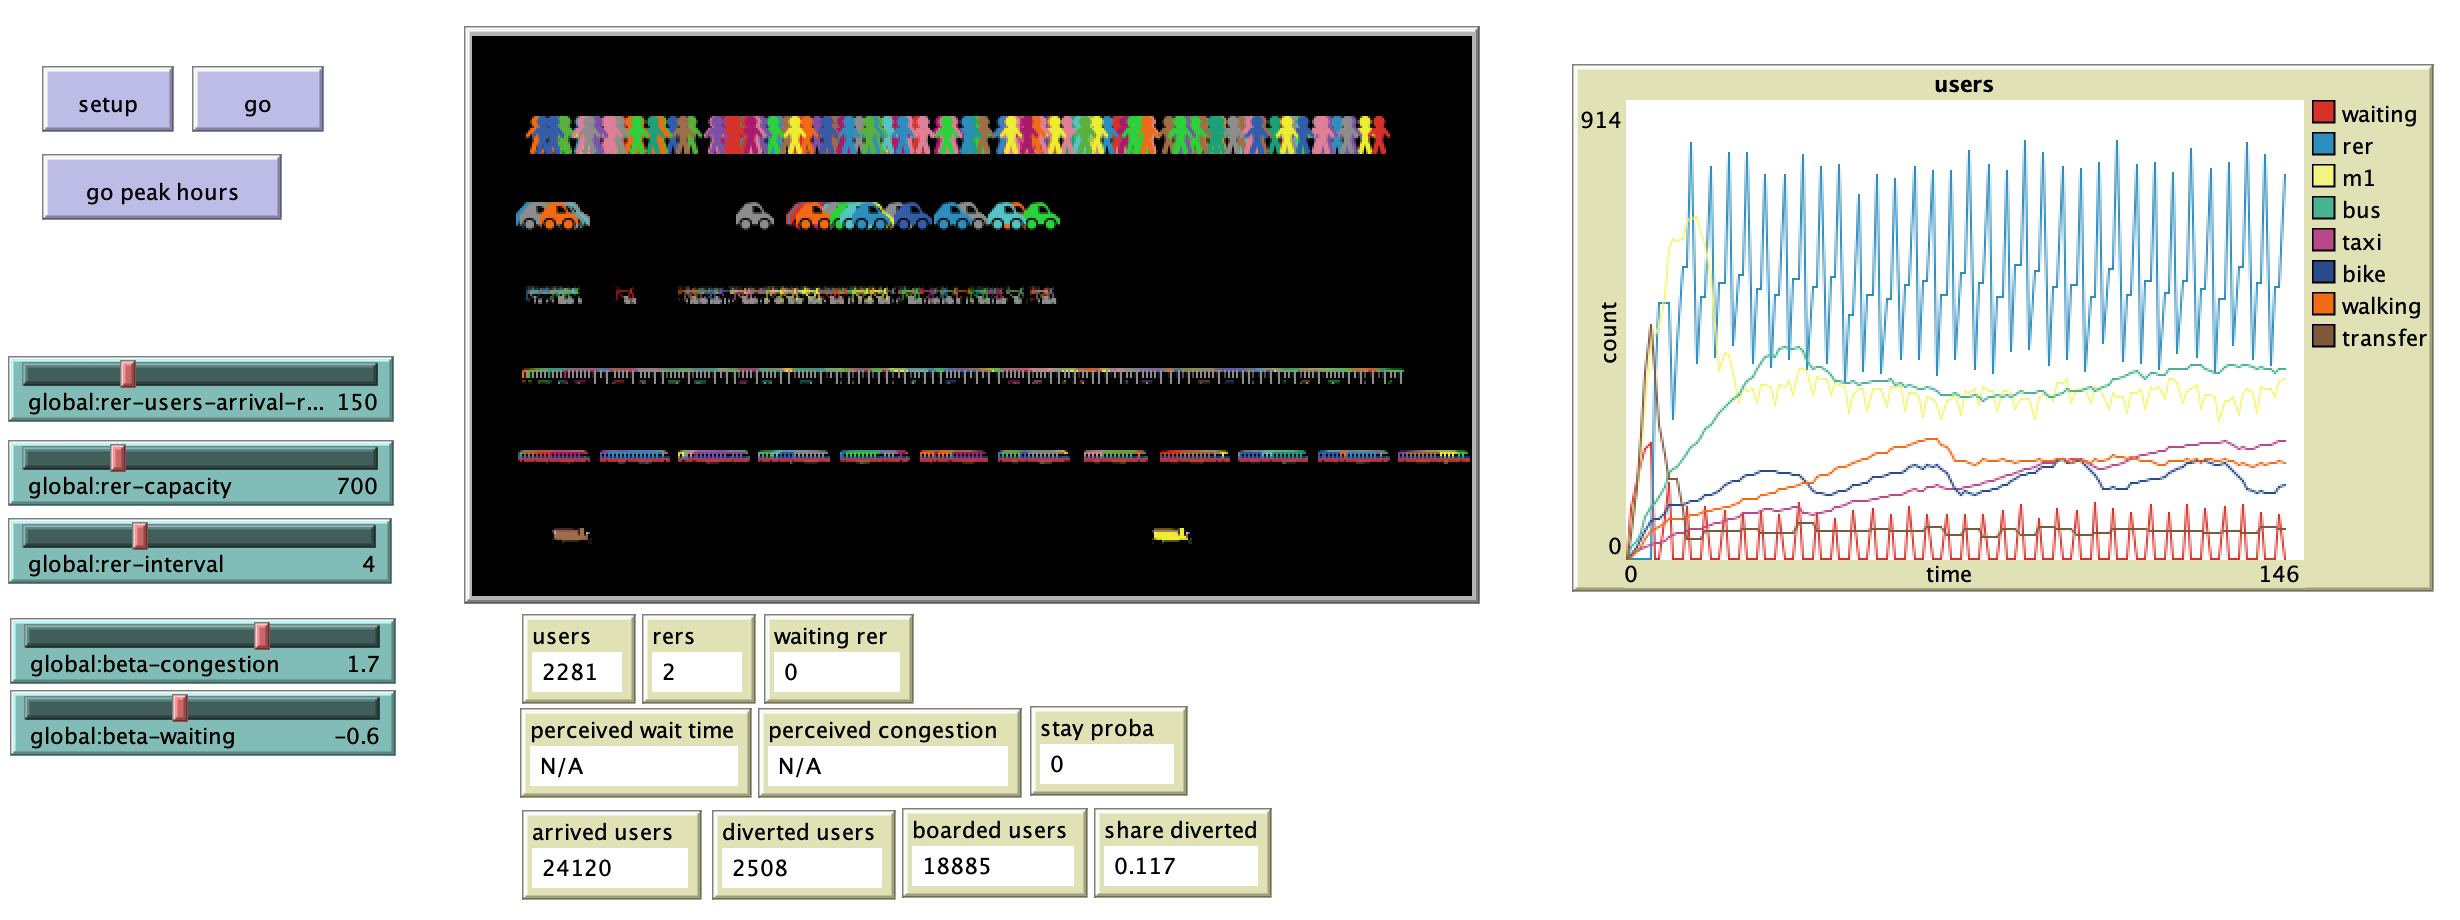
\includegraphics[width=\linewidth]{figures/Fig2.png}}
%\caption{Model interface}
%\end{figure}
%%%%%%%%%%%%

%\section{Model exploration}


%%%%%%%%%%%%
\begin{figure}[t]\vspace*{4pt}
\centerline{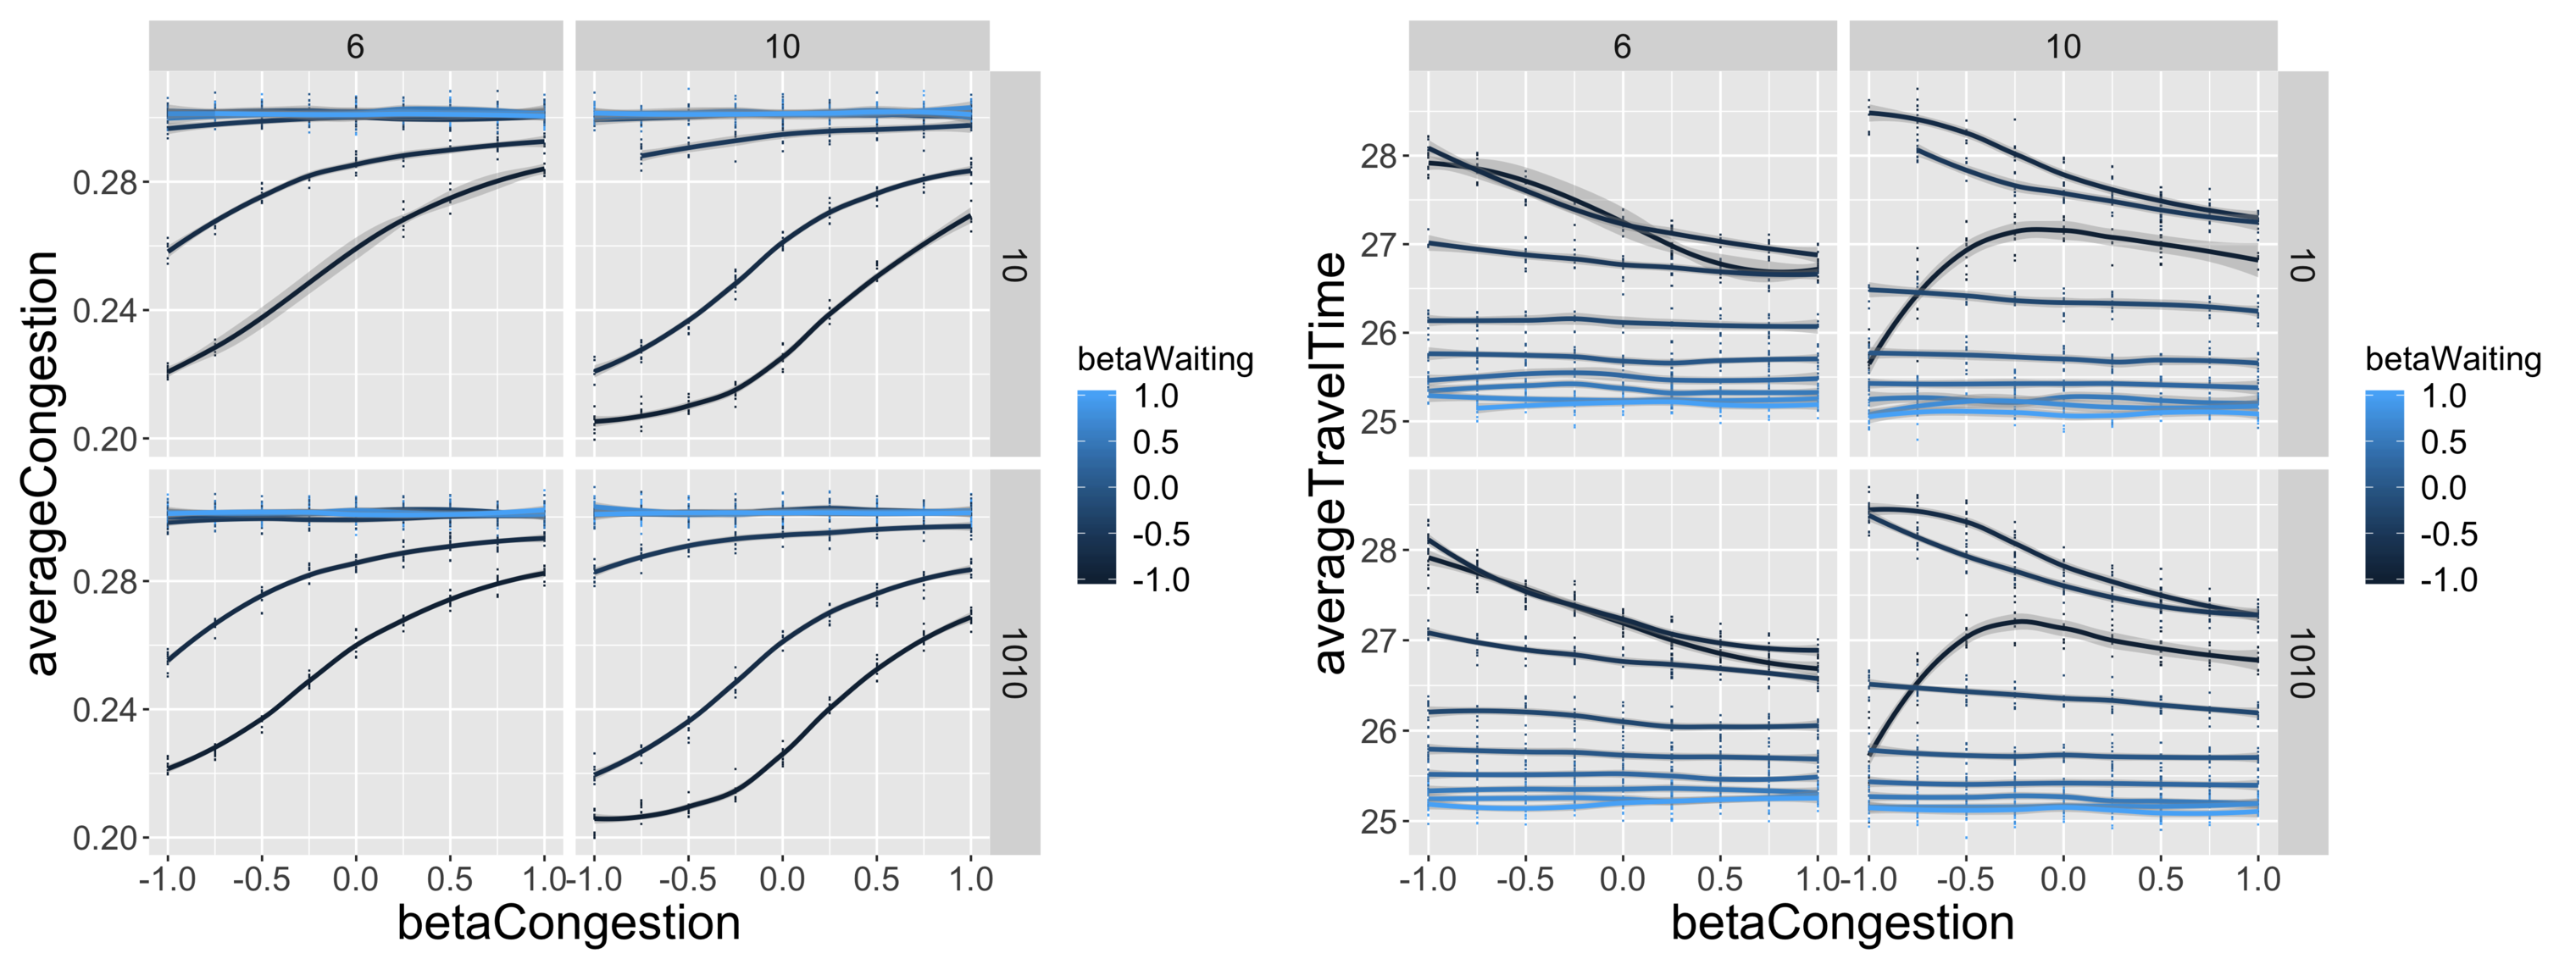
\includegraphics[width=0.6\linewidth]{figures/Fig3.png}}
\caption{Model exploration results. \textit{(Left)} Average congestion as a function of $\beta_c$, for varying $\beta_{\tau}$ (colour), train interval (columns) and train capacity (rows); \textit{(Right)} Average travel time for same parameter values.\label{fig:fig3}}
\end{figure}
%%%%%%%%%%%%





The model is implemented in NetLogo which is specifically suited for such agent-based simulations. The open-source code of the model and results is available as a git repository at \url{https://github.com/JusteRaimbault/ReportMasse}. We systematically explored model parameter space by using the OpenMOLE model exploration software \citep{reuillon2013openmole}, which allows embedding any type of model, provides a seamless access to high performance computing infrastructures, and integrates state-of-the-art model validation and exploration methods. We run 10 stochastic repetitions of the model, for parameters $\beta_c,\beta_{\tau}$, train capacity, train arrival interval within a grid, corresponding to $\simeq 24,000$ runs of the model. We show in Fig.~\ref{fig:fig3} the variation of average travel time and congestion as a function of $\beta_c$. We find an interesting non-linear behavior of travel time for low values of $\beta_{\tau}$ (dark blue, right column), where travel time is maximal around a neutral position of users to congestion: in that context of a low tolerance to waiting, either a low or high tolerance to congestion are better than being indifferent. Regarding congestion, it increases with both discrete choice parameters but differently in the various disruption scenarios.

These preliminary results show how this model can be applied to explore complex congestion patterns in the stylised network following interactions between different components of user behavior. Work in progress includes the application of a genetic algorithm for optimization to the model with the aim to explore compromises between congestion in the train and congestion in alternative modes.


%\section{Discussion}


%% References
%%
%% Following citation commands can be used in the body text:
%% Usage of \cite is as follows:
%%   \cite{key}         ==>>  [#]
%%   \cite[chap. 2]{key} ==>> [#, chap. 2]
%%

%The citation must be used in following style: \cite{article-minimal} \cite{article-full} \cite{article-crossref} \cite{whole-journal}.
%% References with BibTeX database:

%

\vspace{-0.5cm}

\bibliographystyle{elsarticle-harv}
\bibliography{biblio.bib}

\clearpage


\end{document}

%%%%
% Template

%
%\begin{figure}[t]\vspace*{4pt}
%%\centerline{\includegraphics{fx1}\hspace*{5mm}\includegraphics{fx1}}
%\centerline{\includegraphics{gr1}}
%\caption{(a) first picture; (b) second picture.}
%\end{figure}
%
%\begin{table}[h]
%\caption{An example of a table.}
%\begin{tabular*}{\hsize}{@{\extracolsep{\fill}}lll@{}}
%\toprule
%An example of a column heading & Column A ({\it{t}}) & Column B ({\it{t}})\\
%\colrule
%And an entry &   1 &  2\\
%And another entry  & 3 &  4\\
%And another entry &  5 &  6\\
%\botrule
%\end{tabular*}
%\end{table}
%



%
%\begin{equation}
%\begin{array}{lcl}
%\displaystyle X_r &=& \displaystyle\dot{Q}^{''}_{rad}\left/\left(\dot{Q}^{''}_{rad} + \dot{Q}^{''}_{conv}\right)\right.\\[6pt]
%\displaystyle \rho &=& \displaystyle\frac{\vec{E}}{J_c(T={\rm const.})\cdot\left(P\cdot\left(\displaystyle\frac{\vec{E}}{E_c}\right)^m+(1-P)\right)}
%\end{array}
%\end{equation}
%
%



%% The Appendices part is started with the command \appendix;
%% appendix sections are then done as normal sections
%% \appendix

%% \section{}
%% \label{}
%
%\appendix
%\section{An example appendix}
%Authors including an appendix section should do so before References section. Multiple appendices should all have headings in the style used above. They will automatically be ordered A, B, C etc.
%
%\subsection{Example of a sub-heading within an appendix}
%There is also the option to include a subheading within the Appendix if you wish.
%



%
%
%\section*{Acknowledgements}
%
%Acknowledgements and Reference heading should be left justified, bold, with the first letter capitalized but have no numbers. Text below continues as normal.
%

